\documentclass[UTF8]{ctexart}
\usepackage{graphicx}
\usepackage{amssymb}
\usepackage{subfiles}
\usepackage{amsmath}
\usepackage[margin=1in]{geometry}
\begin{document}
\section{Appendix A:The test of the slamming of Mark-III panel}
\paragraph{\quad}In this section, the slamming of the Mark-III type insulation panel carried 
                out by Marrone et al. (2017) is tested. The sketch of the numerical model is shown in Fig. 17. 
                In order to save the computational cost, this panel was initially placed 0.56 m above the water 
                surface. The impact velocity and the deadrise angle of the panel are $U_{impact} = 6m/s$ and $\theta = 4^\circ$,
                respectively. In the present simulation, the particle spacing $\Delta x $is set to 0.002 m. Different from 
                the use of Mach number Ma = Uimpact/cwater = 0.1 in Marrone et al. (2017), Ma = Uimpact/cwater = 0.015 
                is adopted in the present simulation. Similar to Marrone et al. (2017), for easy to compare, the time 
                coordinate of the numerical results is translated to make it consistent with the experimental data in 
                Marrone et al. (2017).
\paragraph{\quad}在本节中,实验了Marrone et al.(2017)提出的Mark-III型绝缘板的砰击。数值模型的示意图如Fig. 17所示。
                为节省计算开销,该板初始被放置在距水面0.56m的高度。板的砰击速度和静升角分别为$U_{impact} = 6m/s$和 $\theta = 4^\circ$。
                在当前模拟中,粒子的间距$\Delta x$设置为0.002m.与Marrone et al.(2017)所用的马赫数$Ma=U_{impact}/c_{water}=0.1$不同,
                本次采用了$Ma=U_{impact}/c_{water}=0.015$.和Marrone er al.(2017)类似,为便于比较,平移了数值结果的时间坐标,使之与
                实验数据(2017)相一致。
{
    \centering
    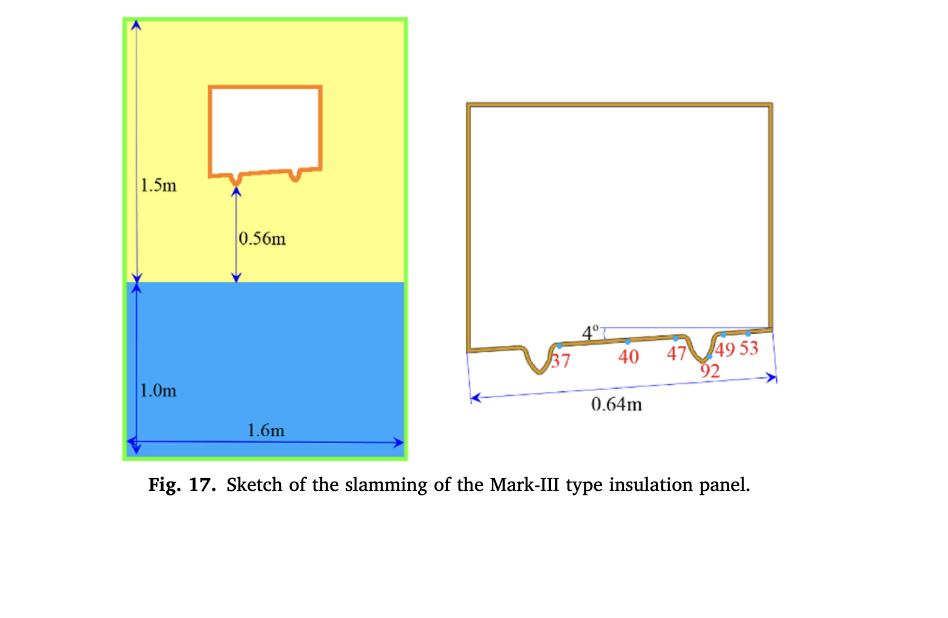
\includegraphics{./source/Fig17.png}
}
\paragraph{\quad}Fig. 18 shows the particle distributions and corresponding pressure fields at three 
                typical time instants. It can be observed that when the left corner of the panel impacts 
                the water, a violent impact pressure wave is produced. With the fall of the panel, the 
                trapped air forms a bubble under the panel. Since the air inside the bubble is compressed, 
                a small high-pressure area is formed under the panel. As the air bubble expands and overflows 
                from the right dent, the bubble pressure becomes lower. In general, the present results can 
                capture the flow pattern of the air cushion under the panel and obtain a relatively smooth 
                pressure field. However, when the water slams onto the structure, there are some pressure 
                noise generated in the local area.
\paragraph{\quad}Fig. 18给出了三个典型时刻的粒子分布和相应的压力场信息。可以看到当板的左角砰击到水面,产升了猛烈的砰击压力波。
                随着板的下落,被困的空气在板下形成了气泡。由于气泡内空气被压缩,一小片高压区域在板下形成。当气泡膨胀并从右齿处
                逸出,气泡内压力变低。总而言之,本文的结果可以捕捉板下气垫的流动模式和相对光滑的压力场。然而,当水砰击到结构物时,
                在局部区域会形成一定的压力噪声。
{
    \centering
    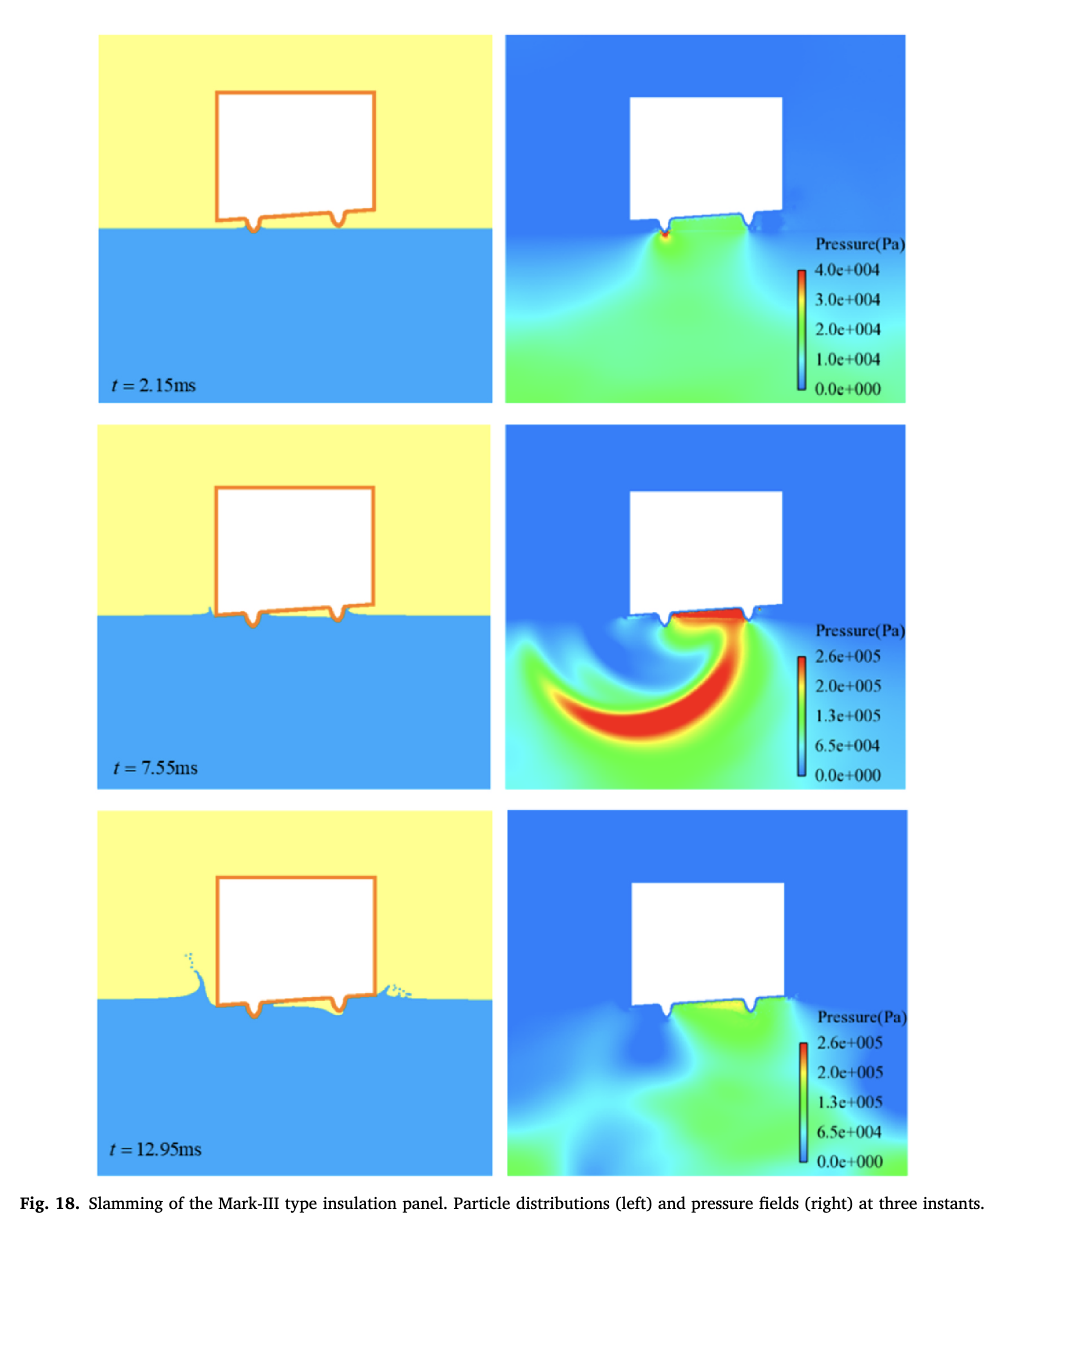
\includegraphics{./source/Fig18.png}
}

\paragraph{\quad}Fig. 19 gives the time histories of the pressure of the six measuring points on the panel, 
                and it can be found that generally, compared with the Riemann-ALE SPH results of 
                Marrone et al. (2017), the pressure peaks of measuring points predicted by the present 
                SPH are larger and the pulse widths are smaller, which are closer to the experimental 
                results of Marrone et al. (2017). This can be attributed to two reasons. On the one hand, 
                a larger water speed of sound is adopted in the present simulation with respect to the one 
                used by Marrone et al. (2017). Therefore, the compressibility of water is weaker in the 
                present work, and when the structure impacts on the water, the present pressure time histories 
                are relatively sharper with larger peak values. On the other hand, owing to the use of the 
                dissipation limiter, the dissipation introduced by the Riemann solver is reduced greatly, and 
                the numerical viscosity of fluid is lower in the present simulation, which also increases the 
                pressure peaks to some extent. However, compared with the smooth pressure evolution obtained 
                by Riemann-ALE SPH in Marrone et al. (2017)Marrone et al. (2017), more severe oscillations are 
                displayed in the present results, especially for the measuring points 49, 53 and 92, which can 
                also be attributed to the adopted larger water speed of sound and the use of the dissipation 
                limiter in the present Riemann SPH.
\paragraph{\quad}Fig. 19给出了板上六个测量点压力的时间历程,可以看出,总体上,与Marrone et al.(2017)的黎曼-ALE SPH结果相比,
                本文SPH方法预测的测量点压力峰值更大且脉冲宽度更小,更接近于Marrone et al(2017)的实验数据。这可以归因于两个原因。
                一方面是本文的模拟使用了比Marrone et al. (2017)所使用的更大的水声速。因此,在本文中水的可压缩性更弱,当结构物砰击
                水时,本文的压力时间历程相对尖锐,峰值较大。另一方面,因为使用了耗散限制器,极大减少了由黎曼求解器产生的好散,并且当前模拟
                中的数值粘度更低,这在一定程度上也增大了压力峰值。然而,与Marrone et al.(2017)中的黎曼-ALE SPH所获得的光滑压力变化相比,
                本文的结果给出了更严重的震荡,特别是对于测量点49,53和92,这也可以归因于在当前SPH方法中应用了更高的水声速和使用了耗散限制器。
{
    \centering
    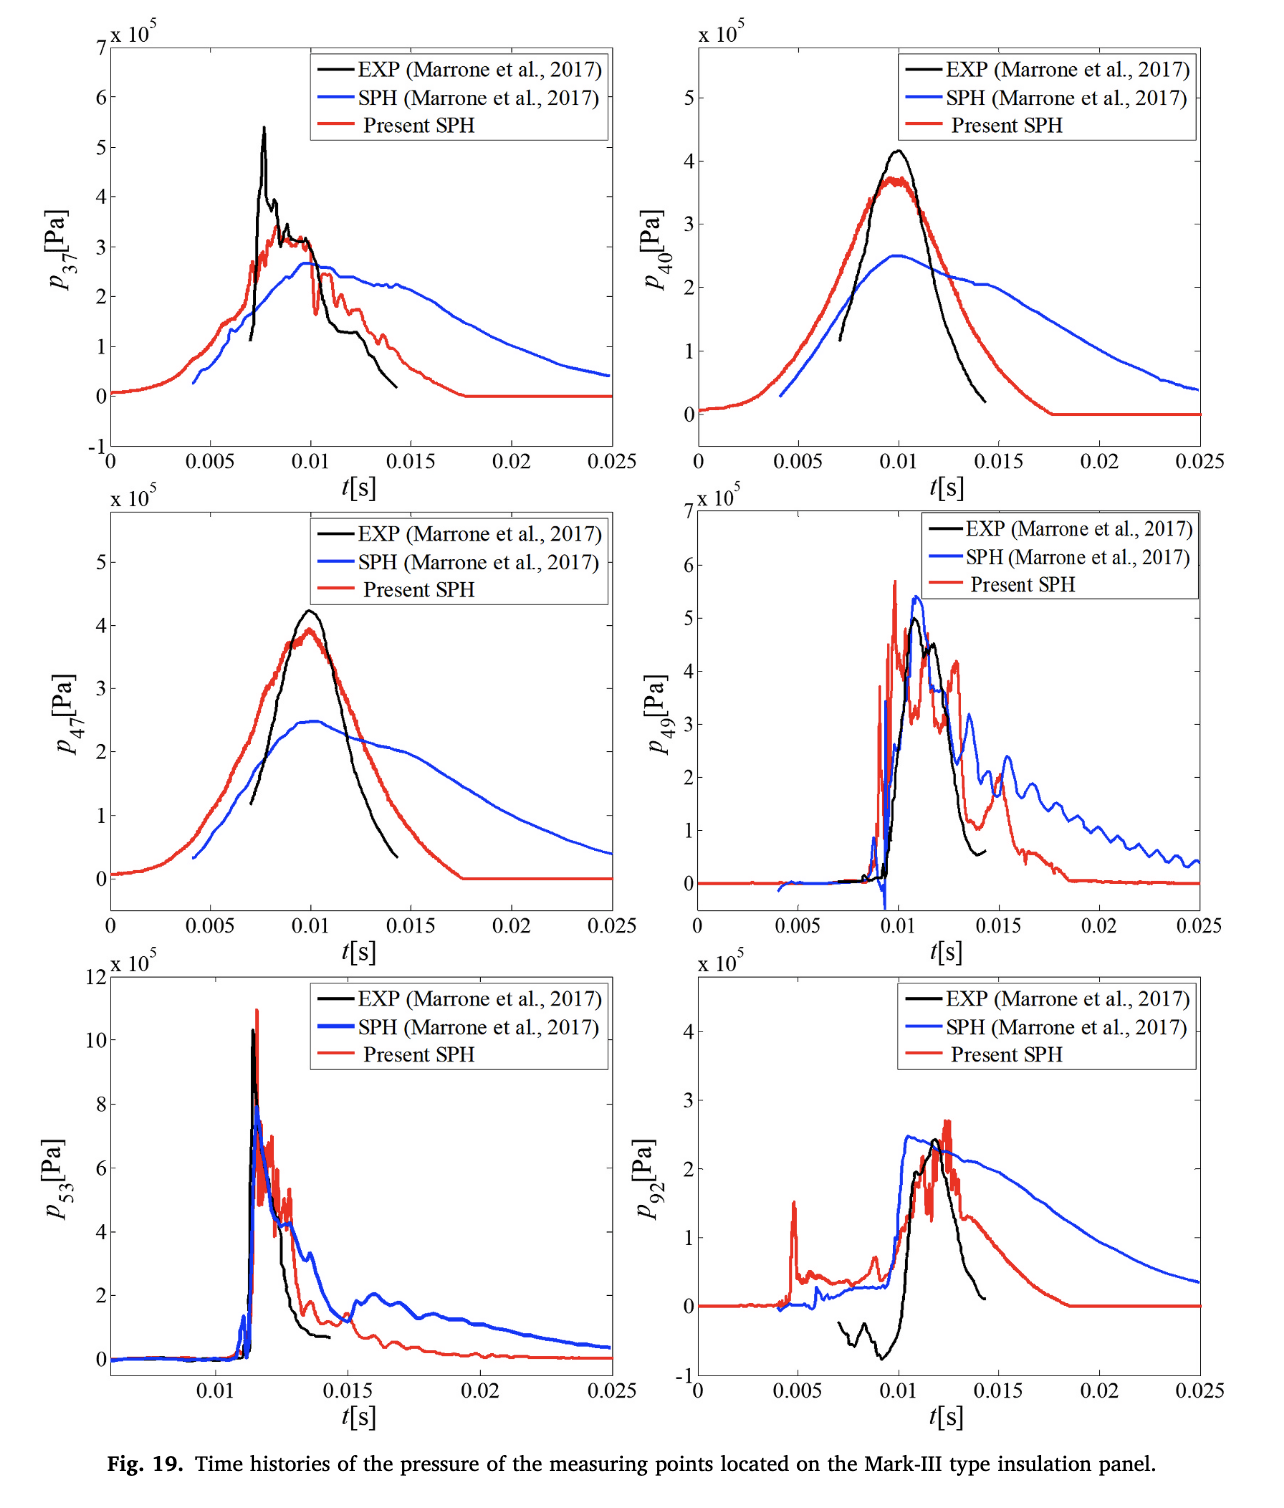
\includegraphics[width=30em]{./source/Fig19.png}
}
{
    \centering
    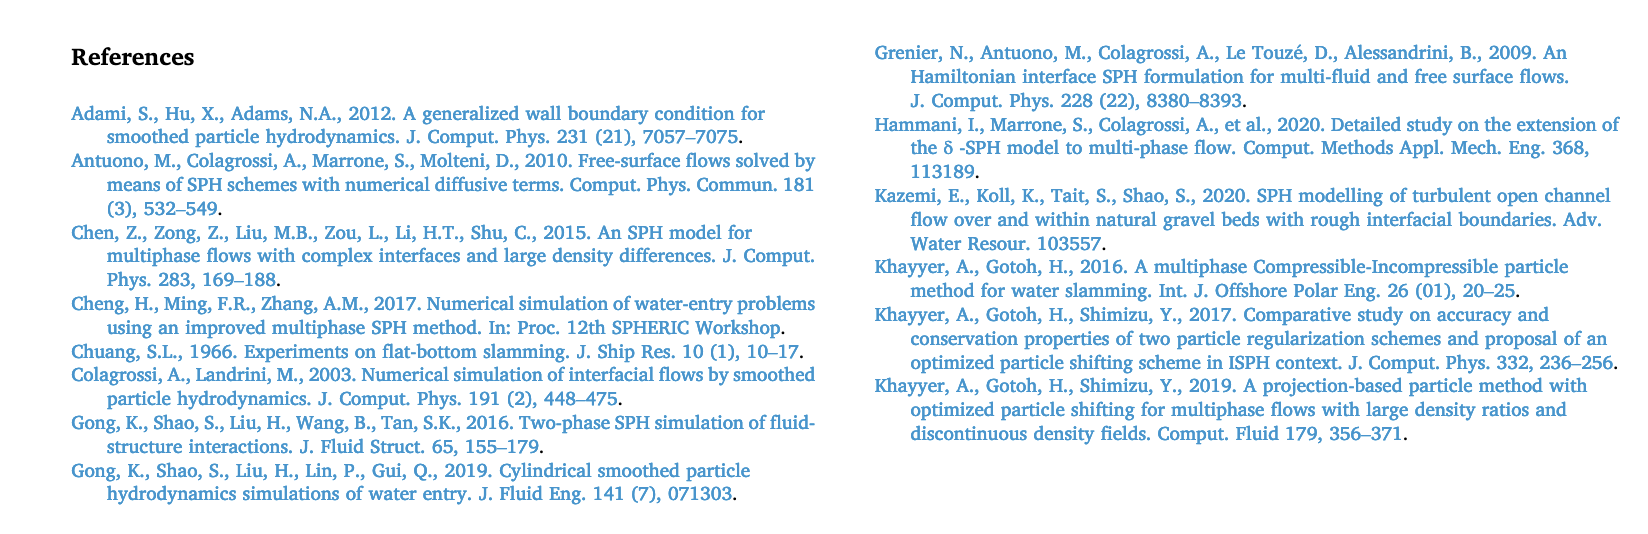
\includegraphics[width=50em]{./source/Fig20.png}\\
    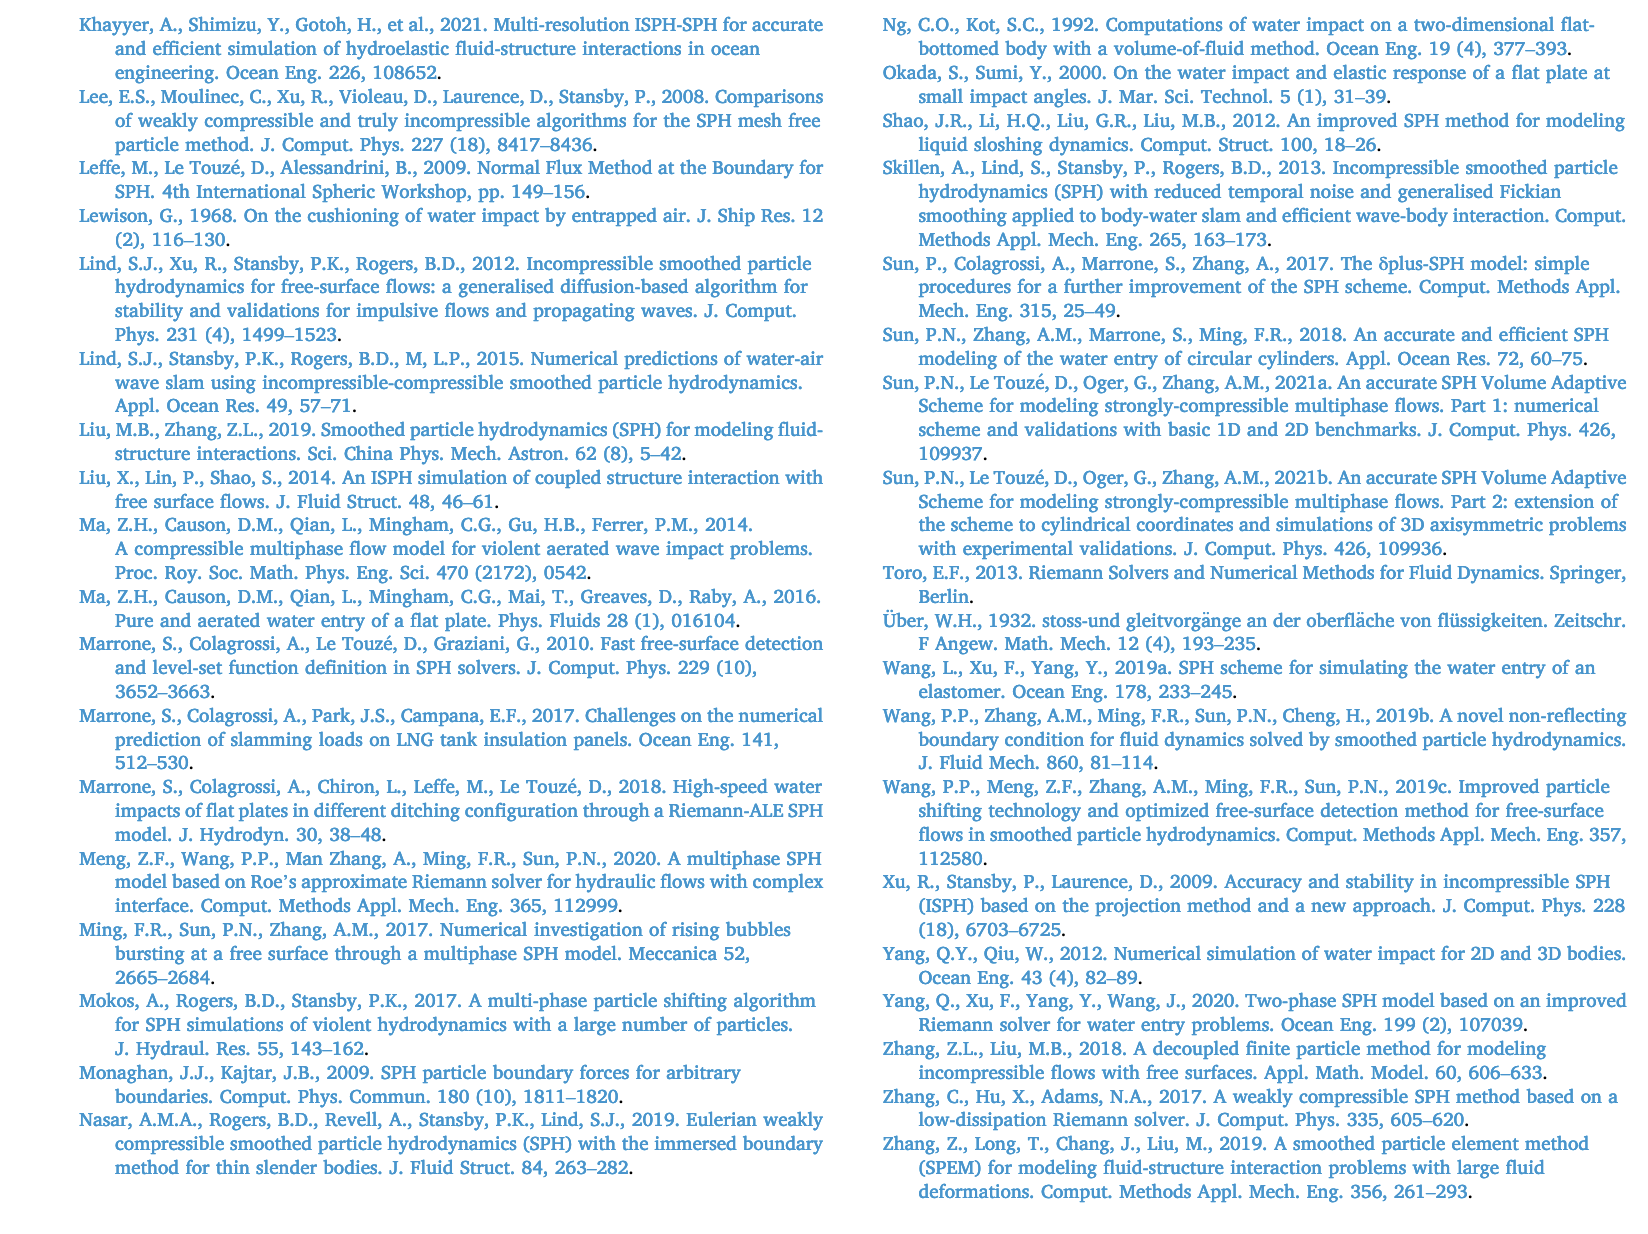
\includegraphics[width=50em]{./source/Fig21.png}
}
\end{document}